
\chapter{Input Layer or Grid Structure Models}\label{chapter-media}

\markright{CHAPTER \ref{chapter-media} MEDIA}

One major reason to use a computational expensive grid-based seismic wave numerical code
is to simulate seismic wave propagation in complex velocity models,
which can significantly affect the seismic waveforms.
The velocity structure of the Earth, especially near the surface, is vey complex.
How to input the complex velocity model and accurately representing 
the velocity model using the discrete simulation grid are important
components of a seismic wave simulation program.

CGFD3D designs two types of file formats to ease the input of the velocity models.
\begin{itemize}
  \item One is the layer-based model format (.md3lay),
which can be used for topographic layers with known medium paramters along the ingterface and vertical gradients for values inside the layer.
  \item The second one is the grid-based model (.md3grd), which is indeed a hybrid model format that also supports topographic layers structures,
but internal value is interpolated from vertically discrete sampling values inside one layer.
Regular grid models produced by tomography, can be taken as a special case of the .md3grd 
with a single layer and equal vertical invertal at all horizonal sampling points.
\end{itemize}
%support two types of the velocity structure models: layer-based and grid-based.
%The layer-based velocity model can be used for topographic layers 
%  with known medium paramters along the ingterface and vertical gradients for values inside the layer.
%While the grid-based model is indeed a hybrid model format that also supports topographic layers structures,
%but internal value is interpolated from vertically discrete sampling values inside one layer.
%Common grid model, such as results by tomography, 
%The grid-based model 


%===============================================================================
\section{Different Medium Types Supported by CGFD3D} \label{sec_medium_type} 
%===============================================================================

CGFD3D supports simulating wave propagation in following media:
 % TODO: waveform eqn. should be given and analyzed before
\begin{itemize}
    \item \texttt{acoustic\_iso}: abbrevation of acoustic wave equation of isotropic media.  
    \item \texttt{elastic\_iso}: abbrevation of elastic wave equation of isotropic media.
    \item \texttt{elastic\_vti}: abbrevation of elastic wave equation of vertical transversely isotropic media. 
    \item \texttt{elastic\_aniso}: abbrevation of elastic wave equation of anisotropic media. 
\end{itemize}
More complex media will be implemented in the future.

%===============================================================================
\section{Medium Parameterization Methods} \label{equivalent_method} 
%===============================================================================

One parameter the user should determine but the meaning is not so straightfowrad is ``medium parameterization method''.
We explain this concept first to ease description of the medium input in following chapters.

If there are topographic interfaces with strong velocity contrast, 
medium paramters at a grid point directly taking values according to its coordinate in the input velocity model
 will result in stair-case representation of the interfaces, introduce interface-related errors and cause stong artificial diffraction.
One advance feathure of CGFD3D is to evaluate equivalent medium parameters at grid points 
to accurately represent the location of the interface inside a grid cell 
and realize subgrid resolution of the layer velocity models.
CGFD3D supports various medium parameterization approaches:
\begin{itemize}
\item loc: \\
  abbrevation of direct location, which is the simplest and most widely used one. 
      In this approach, the medium parameter of a grid point,
      is the value just at that ccoordinate position
      in the input velocity model. In terms of processing time,
      LOC method is fastest comparing to rest methods.
\item ari: \\
  abbrevation of volume arithmetic averaging (add ref) as
  \begin{align}
    \left<var\right> = \frac{1}{\Delta V} 
            \int_{k-1/2}^{k+1/2} \int_{j-1/2}^{j+1/2} \int_{i-1/2}^{i+1/2} var~dx dy dz,
  \end{align}
  which evaluats an averaging value for all the medium parameters
    in the cell volume representing by the grid point.
\item har: \\
  abbrevation of volume harmonic averaging for medium modulus as 
  \begin{align}
    \left<var\right>^H = \frac{\Delta V}
      {\int_{k-1/2}^{k+1/2} \int_{j-1/2}^{j+1/2} \int_{i-1/2}^{i+1/2} \frac{1}{var} dx dy dz},
  \end{align}
  which evaluats an averaging value of medium modulus in the cell volume representing by the grid point,
  while and volume arithmetic average for density as proposed by (ref).
  The approach does not alter medium type,
    e.g., isotropic model is still an isotropic one, after parametrization.
\item tti: \\
  abbrevation of tiled transversely isotropic equivalent medium approach (add ref), 
        which evaluats an effictive TTI representation of the thin layers inside the cell volume representing by the grid point.
        The approach does alter medium type, e.g., isotropic model becomes a TTI anisotropic one, after parametrization.
\end{itemize}


The parametrization name may mean a slightly different combination of hormonic and arithmetic
averaging of difference medium parameters for different medium types (Table~\ref{table_parameterization}).

\begin{table}[h!]
\centering
\begin{tabular}{| c | c | c | c | c |}
\hline
   medium type               &   loc$^L$   &   ari$^A$   & har$^H$  & tti$^T$ \\
\hline
   \verb|one_component|      &    all$^L$  &   all$^A$   & all$^H$  &  NA \\
\hline
   \verb|acoustic_isotropic| &    all$^L$  &   all$^A$   &$\kappa^H$, $\rho^A$ & todo \\
\hline
   \verb|elastic_isotropic|  &    all$^L$  &   all$^A$   &$\lambda^H$,$\mu^H$,$\rho^A$ &  todo \\
\hline
   \verb|elastic_vti_*|      &    all$^L$  &   all$^A$   &$C_{ij}^H$, $\rho^A$ & todo \\
\hline
   \verb|elastic_aniso_cij|  &    all$^L$  &   all$^A$   &$C_{ij}^H$, $\rho^A$ & todo \\
\hline
   \verb|elastic_tti_*|      &    all$^L$  &   all$^A$   &$C_{ij}^H$, $\rho^A$ & todo \\
\hline
\end{tabular}
\caption{Medium parameterization on difference parameters for different medium types.}
\label{table_parameterization}
\end{table}

%\begin{table}[h!]
%\centering
%\caption{Medium parameterization on difference parameters for different medium types.}
%\label{table_parameterization}
%\begin{tabular}{| c | c | c | c | c | c |}
%\hline
%   medium type  &   \verb|one_component|    &   \verb|acoustic_isotropic| & \verb|elastic_isotropic|
%                &  \verb|elastic_vti_*| & \verb|elastic_aniso_cij/elastic_tti_*| \\
%\hline
%    loc    &   as is  &  as is  &     as is  &     as is  &     as is  \\
%\hline
%  ari$^A$  &   as is  &  as is  &     as is  &     as is  &     as is  \\
%\hline
%   har$^H$ &   as is &  $\kappa^H$, $\rho^A$  &  $\lambda^H$,$\mu^H$,$\rho^A$
%             &     $C_{ij}^H$, $\rho^A$  &  $C_{ij}^H$, $\rho^A$  \\
%\hline
%  tti      &   NA &   NA &   NA &   NA &   NA \\
%\hline
%\end{tabular}
%\end{table}


%If the media type in the \textbf{md3grd} or \textbf{md3lay} file is \texttt{one\_component}, \texttt{equivalent\_medium\_method} can be
%\begin{itemize}
% \item \texttt{loc}: using local value to discrete model. 
% \item \texttt{ari}: volume integral arithmetic average. 
% \item \texttt{har}: volume integral harmonic average, 
%\end{itemize}
%
%If the media type is \texttt{acoustic\_isotropic}, \texttt{equivalent\_medium\_method} can be
%\begin{itemize}
% \item \texttt{loc}: using local media parameters to discrete model. 
% \item \texttt{har}: applying harmonic average to $\kappa$, and applying arithmetic average to density $\rho$. 
% \item \texttt{ari}: applying arithmetic average to $\kappa$ and $\rho$. 
%\end{itemize}
%
%If the media type is \texttt{elastic\_isotropic}, \texttt{equivalent\_medium\_method} can be
%\begin{itemize}
% \item \texttt{loc}: using local media parameters to discrete model. 
% \item \texttt{har}: applying harmonic average to elastic modulus, and applying arithmetic average to density $\rho$. Please see \citet{moczo_3d_2002} and \citep{moczo_finite-difference_2014} for detail.
% \item \texttt{ari}: applying arithmetic average to elastic modulus and density. 
%\end{itemize}
%
%If the media type is \texttt{elastic\_vti\_*}, \texttt{equivalent\_medium\_method} can be
%\begin{itemize}
% \item \texttt{loc}: using local media parameters to discrete model. 
% \item \texttt{har}: applying harmonic average to elastic modulus $c_{ij}$, and applying arithmetic average to density $\rho$.
% \item \texttt{ari}: applying arithmetic average to elastic modulus $c_{ij}$ and density. 
%\end{itemize}
%
%If the media type is \texttt{elastic\_aniso\_cij} or \texttt{elastic\_tti\_*}, \texttt{equivalent\_medium\_method} can be
%\begin{itemize}
% \item \texttt{loc}: using local media parameters to discrete model. 
% \item \texttt{har}: applying harmonic average to elastic modulus $c_{ij}$, and applying arithmetic average to density $\rho$.
% \item \texttt{ari}: applying arithmetic average to elastic modulus $c_{ij}$ and density. 
%\end{itemize}

%===============================================================================
\section{Parameters in Main Par File} \label{sec_medium_json} 
%===============================================================================

\begin{lstlisting}[language=json,
    label={lst_medium_json},
    caption=Example of medium settings in .json,
    frame=tb]
  "medium" : {
      "type" : "elastic_iso",
      "#code" : 1,
      "infile_layer" : "/home/usr1/testCGFD3D/prep_medium/basin.md3lay",
      "#infile_grid" : "/home/usr1/testCGFD3D/prep_medium/basin.md3grd",
      "#equivalent_medium_method" : "har",
      "#import" : "/home/usr1/testCGFD3D/output/media"
  },
  "is_export_media" : 1,
  "media_export_dir"  : "/home/usr1/testCGFD3D/output/media",

  "#visco_config" : {
      "type" : "graves_Qs",
      "Qs_freq" : 1.0
  }
\end{lstlisting}

There are several medium related keys in the main par .josn file (List~\ref{lst_medium_json}),
\begin{itemize}
\item \verb|medium|: \\
  major block for medium input, tells the program:
  \begin{itemize}

  \item \texttt{type} determins the solver equation, that is,
    what medium you want to simulate wave propagation in.
    Four options are currently supported in this code:
    \begin{itemize}
      \item \texttt{acoustic\_iso}: acoustic wave equation of isotropic media,
      \item \texttt{elastic\_iso}: elastic wave equation of isotropic media,
      \item \texttt{elastic\_vti}: elastic wave equation of vertical transversely isotropic media,
      \item \texttt{elastic\_aniso}: elastic wave equation of anisotropic media. 
    \end{itemize}

  \item how the structure model is input or specified.
    There are four possible ways:
    \texttt{import}, \texttt{code}, \texttt{infile\_layer} or \texttt{infile\_grid}.
    \begin{itemize}  
      \item \texttt{code}: \\
        Choose this flag if you want to give the media by code.
                 You should edit \textbf{forward/md\_t.c} file and recompile the code.
      \item \texttt{infile\_layer}: \\
        If you want to give media by the intereface line,
          this option should be helpful. The media parameters are given by the \textbf{md3lay} file,
          and the file format is shown in Section \ref{md3lay} 
      \item \texttt{infile\_grid}: \\
        If you want to give media by a given grid media,
          this option should be helpful. The media parameters are given by the \textbf{md3grd} file,
          the file format is shown in Section \ref{md3grd}.
      \item \texttt{import}: \\
        If you already generated media from the above three options,
        and do not want to re-generate media, 
        select this option and give the folder of the exported media. 
    \end{itemize}

  \item \texttt{equivalent\_medium\_method}: If you specify structure mode by
        \texttt{infile\_layer} or \texttt{infile\_grid},
        equivalent medium parameterization methods can be applied.
        For different media, we provide different equivalent medium parameterization methods,
        please see Section \ref{equivalent_method} for detail.
  \end{itemize}
   
\item \verb|is_export_media|: \\
  if the discreted medium parameters at FD grid points are exported 
       for display purpose or reuse for later calculation without re-discrete media calculation.
    \begin{itemize}
      \item 0: do not export discrete media,
      \item 1: export discrete media.
    \end{itemize}
\item \verb|media_export_dir|: \\
  set the output dir if \verb|is_export_media : 1|.
  
\item \verb|visco_config|: \\
  block for attuantion settings.
  If this block is enabled (appeared in the .json),
    the attuation will be implemented with following two parameters (add Grave's ref):
  \begin{itemize}
    \item \verb|type|: currently only \verb|graves_Qs| can be set, which means to implement
       attuation following Grave (1996) approach.
     \item \verb|Qs_freq|: the frequency of the wavefield for which 
          the Q effect is most accurately approximated.
  \end{itemize}

\end{itemize}


%===================================================================
\section{Format of Layer-based Velocity Model (.md3lay)} \label{md3lay}
%===================================================================

The Earth structure of many regions has following features:
\begin{itemize}
  \item the structure consists of many layers with topographic interfaces,
  \item the velocity or density in some layers may increase or decrease along depth,
      which may be expressed by the value at the interface
      and two polynomial parameters (coefficient and power) with respect to depth.
\end{itemize}
For such structures, we can use .md3lay file to input the structure into CGFD3D.


\begin{lstlisting}[language=bash, caption=Example of .md3lay file,
   numbers=left, numbersep=5pt,numberstyle=\tiny\color{codegray}, commentstyle=\color{codegreen},
    label={lst_medium_md3lay},
   frame=tb]
elastic_isotropic
4
126 106 -300.000000 -300.000000 100.000000 100.000000
-0 1000 0.2 1 1500 0.2 1 1000 0.2 1
-0 1000 0.2 1 1500 0.2 1 1000 0.2 1
-0 1000 0.2 1 1500 0.2 1 1000 0.2 1
-0 1000 0.2 1 1500 0.2 1 1000 0.2 1
-0 1000 0.2 1 1500 0.2 1 1000 0.2 1
-0 1000 0.2 1 1500 0.2 1 1000 0.2 1
-0 1000 0.2 1 1500 0.2 1 1000 0.2 1
.
.
.
\end{lstlisting}

\begin{figure}
    \centering
    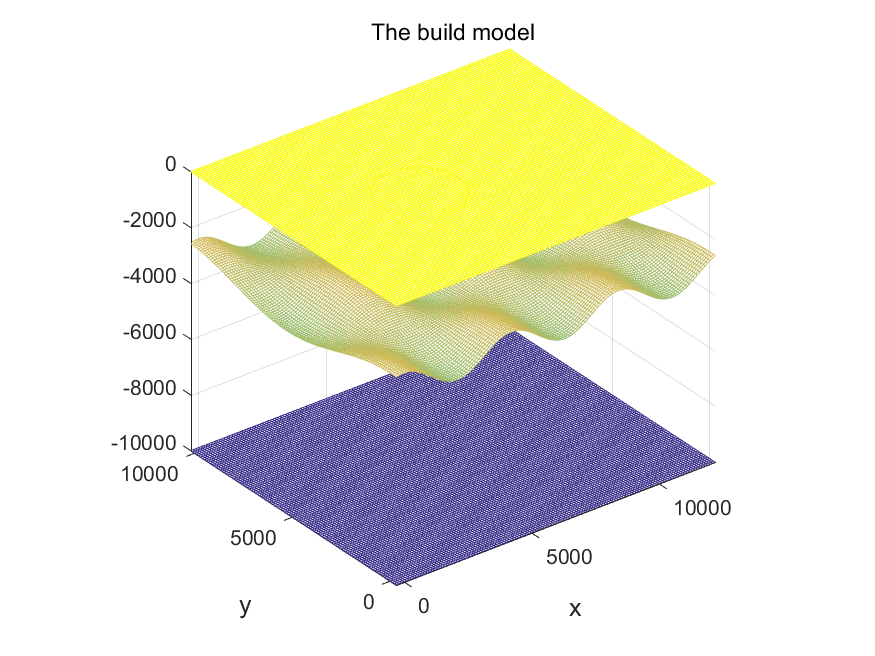
\includegraphics[width=0.5\textwidth]{md3lay_basin.png}
    \caption{Layer-based velocity model with topographic internal interfaces.}
    \label{fig_md3lay}
\end{figure}


An example of .md3lay is shown in Listing~\ref{lst_medium_md3lay} and Figure~\ref{fig_md3lay}.
The detailed format of the .md3lay is:
\begin{itemize}
  \item The first line: sets the medium type, which can be
    \begin{itemize}
    \item \verb|one_component|: \\
      there is only a single medium parameter in this file.
    \item \verb|acoustic_isotropic|: \\
      two parameters $\rho$ and Vp.
    \item \verb|elastic_isotropic|: \\
      three parameters $\rho$, Vp, Vs.
    \item \verb|elastic_vti_prem|: \\
      density and five VTI parameters same to PREM model,
       $\rho$, vph, vpv, vsh, vsv, $\eta$. Please see \citep{dziewonski1981preliminary} for detail.
    \item \verb|elastic_vti_thomsen|: \\
      density and five Thomsen parameters,
        $\rho$, $\alpha_0$, $\beta_0$, $\epsilon$, $\delta$, $\gamma$.
        Please see \citep{ thomsen1986weak} for detail.
    \item \verb|elastic_vti_cij|: \\
      density and five VTI parameters given by $C_{ij}$,
         $\rho$, $c_{11}$, $c_{33}$, $c_{55}$, $c_{66}$, $c_{13}$. 
    \item \verb|elastic_tti_thomsen|: \\
      density ,five Thomsen parameters, two angle of symmetric axis.
         $\rho$, $\alpha_0$, $\beta_0$, $\epsilon$, $\delta$, $\gamma$, $\Phi$, $\theta$.
         Please see \citep{thomsen1986weak} for detail.
    \item \verb|elastic_tti_bond|: \\
          $\rho$, $c_{11}$, $c_{33}$, $c_{55}$, $c_{66}$, $c_{13}$, $\Phi$, $\theta$.
          $\Phi$ is azimuth angle, $\theta$ is the dip angle.
    \item \verb|elastic_aniso_cij|: \\
           $\rho$, $c_{11}$, $c_{12}$, $c_{13}$, $c_{14}$, $c_{15}$, $c_{16}$,  
                                      $c_{22}$, $c_{23}$, $c_{24}$, $c_{25}$, $c_{26}$, 
                                      $c_{33}$, $c_{34}$, $c_{35}$, $c_{36}$, $c_{44}$,
                                      $c_{45}$, $c_{46}$, $c_{55}$, $c_{56}$, $c_{66}$.

    \end{itemize}

  \item The second line: the number of interface (\texttt{NI}) (4 in this example).

  \item The third line:
    six values (two integers and four float) specify the horizontal sampling points as:\\
    \texttt{NX} ~~ \texttt{NY} ~~ \texttt{X0} ~~ \texttt{Y0} ~~ \texttt{DX} ~~ \texttt{DY}, \\
    where
    \begin{itemize}
      \item \texttt{NX} and \texttt{NY}:
          the number of sampling points along $x$ and $y$ direction (126 and 106 for this example);
      \item \texttt{X0} and \texttt{Y0}: 
        the $x$ and $y$ coordinates of the first point (-300 and -300 for this example);
      \item \texttt{DX} and \texttt{DY}:
        spacing between sampling points along $x$ and $y$ (100 and 100 for this example).
    \end{itemize}

 \item 
  Rest are the elevation and media parameters of each sampling point per line.
  Take the \texttt{elastic\_isotropic} media as an example, the media parameters are read as:
  \begin{lstlisting}[language = C]
  for (ni=0; ni<NI; ni++)
    for (iy=0; iy<NY; iy++) 
      for (ix=0; ix<NX; ix++) 
        fscanf(in_3lay_file, "%f %f %f %f %f %f %f", 
               &elevation,
               &rho, &rho_grad, &rho_pow,
               &vp, &vp_grad, &vp_pow,
               &vs, &vs_grad, &vs_pow);
  \end{lstlisting}
  where \texttt{*\_grad} and \texttt{*\_pow} are the coefficient and power of the parameters
    in z-direction as in following equation:
   \begin{equation*}
     \rm{value}^{\rm{grid~point}} = \rm{value}^{\rm{interface}}
        + (z^{\rm{interface}}-z^{\rm{grid~point}})^{var\_pow} * var\_grad.
   \end{equation*}
   Please notice that the z-axis is positive upward in CGFD3D.

\end{itemize}

Please note that
\begin{itemize}
  \item if the computational grid point is located above the top interface of the .md3lay model,
the medium parameters are taken as the values at the top interface.
  \item Different media parameters can have different \texttt{*\_grad} and \texttt{*\_pow}.
\end{itemize}

You can find matlab example script to generate .md3lay in \textbf{example/prep\_medium} directory.

%===================================================================
\section{Format of Grid-based Velocity Model (.md3grd)} \label{md3grd}
%===================================================================

If the velocity variation along depth inside a layer can not be expressed by a polynomial expression
with respect to depth, then we have to give sampling values at discrete points along the depth.
This is why we privoide the .md3grd, the grid-based velocity file.

We design the .md3grd also supporting layer interfaces,
thus the interface effects can be simulated as accurate as possible.
To do so, we need to also set number of layers in the .md3grd file,
then discrete the velocity variation along depth for each layer.


\begin{lstlisting}[language=bash, caption=Example of .mdgrd file,
   numbers=left, numbersep=5pt,numberstyle=\tiny\color{codegray}, commentstyle=\color{codegreen},
    label={lst_medium_md3grd},
   frame=tb]
elastic_isotropic
3
 11 21 101
126 106 -300.000000 -300.000000 100.000000 100.000000
0 1000 1510 1020
0 1000 1510 1020
0 1000 1510 1020
0 1000 1510 1020
0 1000 1510 1020
0 1000 1510 1020
0 1000 1510 1020
.
.
.
\end{lstlisting}

%\begin{figure}
%    \centering
%    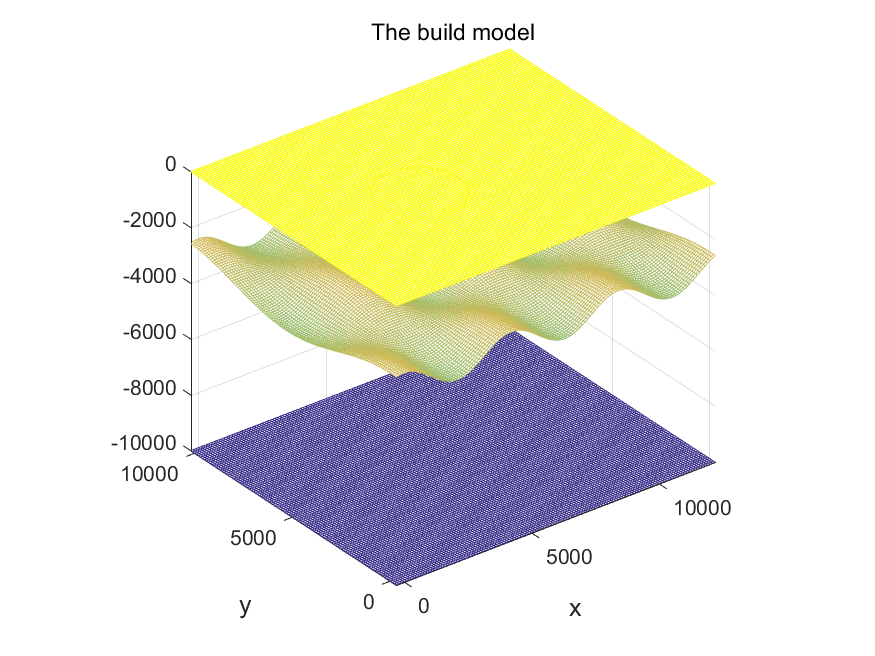
\includegraphics[width=0.5\textwidth]{md3lay_basin.png}
%    \caption{Layer-based velocity model with topographic internal interfaces.}
%    \label{fig_md3grd}
%\end{figure}


An example of .md3grd is shown in Listing~\ref{lst_medium_md3grd}. % and Figure~\ref{fig_md3grd}.
The detailed format of the .md3grd is:
\begin{itemize}
  \item The first line: \\
    sets the medium type, similar to that of .md3lay. 
     Please see descriptions in \ref{md3lay}.

   \item The second line: \\
     is the number of layer or interfaces (\texttt{NL}) (3 in this example).
     If \texttt{NL} = 1, the model becomes the standard grid model that
     only has descrete sampling value along depth but without interfaces.
     If \texttt{NL} > 1, the equivalent medium parameterization can be applied across the interfaces.

   \item The next \texttt{NL} numbers (either at the same line or \texttt{NL} lines)
     set the number of grids in the z-direction of \texttt{NL} layer.
  
   \item The next line: \\
      six values (two integers and four float) specify the horizontal sampling points as:\\
      \texttt{NX} ~~ \texttt{NY} ~~ \texttt{X0} ~~ \texttt{Y0} ~~ \texttt{DX} ~~ \texttt{DY}, \\
      where
      \begin{itemize}
        \item \texttt{NX} and \texttt{NY}:
            the number of sampling points along $x$ and $y$ direction (126 and 106 for this example);
        \item \texttt{X0} and \texttt{Y0}: 
          the $x$ and $y$ coordinates of the first point (-300 and -300 for this example);
        \item \texttt{DX} and \texttt{DY}:
          spacing between sampling points along $x$ and $y$ (100 and 100 for this example).
      \end{itemize}

  \item Rest are the elevation and media parameters of every grid point per line.
    Take the \texttt{elastic\_isotropic} media as an example,
    the media parameters are read as:
  \begin{lstlisting}[language = C]
  for (nl=0; nl< NL; nl++)
    for (ip=0; ip<np[nl]; np++)
      for(iy=0; iy<NY; iy++)
        for (ix=0; ix<NX;ix++)
          fscanf(in_3grd_file, "%f %f %f %f", 
              &elevation, &rho, &vp, &vs);
  \end{lstlisting}
  The medium parameter at a computational grid point is calculated
    by linear interpolation of two values at the discrete velocity model points
    nearest to the computational grid point.

\end{itemize}


Please note that
\begin{itemize}
  \item if the computational grid point is located above the top interface of the .md3grd model,
the medium parameters are taken as the values at the top interface.
  \item if \texttt{NL} > 1, the z-axis of last point of the top layer should be equal to that of
    the first point of the lower layer,
    and the equivalent medium parameterization method can be applied at points close to the interface.
\end{itemize}

You can find matlab example script to generate .md3grd in \textbf{example/prep\_medium} directory.
